% Intended LaTeX compiler: xelatex
\documentclass[10pt, svgnames]{beamer}
\usepackage{graphicx}
\usepackage{longtable}
\usepackage{wrapfig}
\usepackage{rotating}
\usepackage[normalem]{ulem}
\usepackage{amsmath}
\usepackage{amssymb}
\usepackage{capt-of}
\usepackage{hyperref}
\usetheme{metropolis}
\author{Sappinandana Akamphon}
\date{\today}
\title{Shaft and Shaft Components}
\subtitle{ME 310: Mechanical Design}
\usepackage{booktabs}
\usepackage{pgfplots}
\usepackage{multirow}
\usepackage{smartdiagram}
\pgfplotsset{compat=1.18}
\institute{Department of Mechanical Engineering, TSE}
\date{}
\usetikzlibrary{patterns,shapes,arrows}
\AtBeginSection[]{\begin{frame}{Outline}\tableofcontents[currentsection]\end{frame}}
\hypersetup{
 pdfauthor={Sappinandana Akamphon},
 pdftitle={Shaft and Shaft Components},
 pdfkeywords={},
 pdfsubject={},
 pdfcreator={Emacs 30.0.50 (Org mode 9.6)}, 
 pdflang={English}}
\begin{document}

\maketitle

\section{Overview}
\label{sec:org99923cc}

\begin{frame}[label={sec:org2977922}]{Why Starting off with Shafts?}
\begin{itemize}
\item Most engineering machines is powered by a rotational machines
\item Rotational machines need shafts
\item The source of powers\ldots{}  and mistakes
\end{itemize}
\end{frame}

\begin{frame}[label={sec:org4b2bd09}]{Design Criteria}
\begin{itemize}
\item Material selection
\item Layout
\item Stress and strength
\item Deflection and rigidity
\item Vibration
\end{itemize}
\end{frame}

\begin{frame}[label={sec:org26d80b8}]{Materials}
\begin{itemize}
\item Stiffness and deflection: \(E\) same for all steels, so material choice does not matter.
\item Size:

\item For small diameter shafts, use cold drawn steel.
\item If heat treatment is required, it should be machined after to provide work hardening.

\item Production volume:

\begin{itemize}
\item Low \(\rightarrow\) Turning (using lathe or CNC)
\item High \(\rightarrow\) hot rolling, cold rolling, casting
\end{itemize}
\end{itemize}
\end{frame}

\section{Shaft Layout}
\label{sec:orga131834}

\begin{frame}[label={sec:orga4b77e0}]{Layout}
\begin{figure}[htbp]
  \centering
  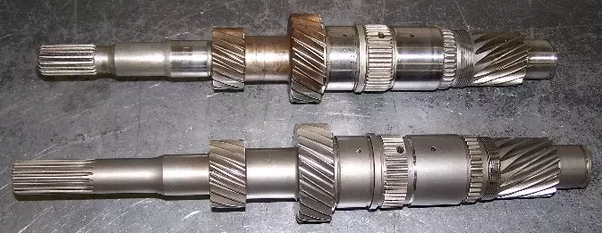
\includegraphics[width=0.8\textwidth]{Pictures/shaft-with-steps}
\end{figure}

\begin{itemize}
\item steps to axially locate elements, i.e. gears, pulleys, bearings.
\item support axial load using bearings
\item provide torque transmission with gears, pulleys, sprockets\ldots{}
\end{itemize}
\end{frame}

\begin{frame}[label={sec:orge667ad8}]{Axial Location of Elements}
\begin{figure}[htbp]
  \centering
  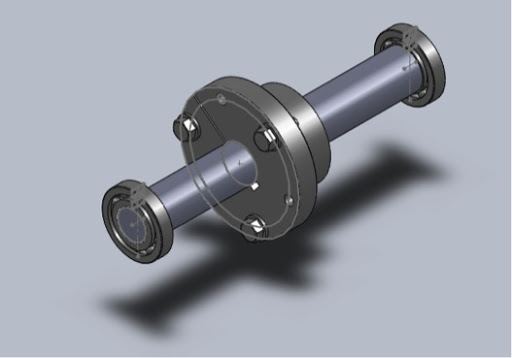
\includegraphics[width=0.7\textwidth]{Pictures/key-steps}
\end{figure}

\begin{itemize}
\item 2 bearings per shaft in most cases
\item Shortest shaft possible to reduce bending
\item Load bearing components should be close to bearings
\item Use shoulders or retainer rings to fix axial locations
\end{itemize}
\end{frame}

\begin{frame}[label={sec:orge461290}]{Axial Load Support}
\begin{figure}[htbp]
  \centering
  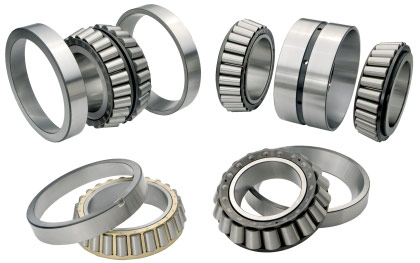
\includegraphics[width=0.7\textwidth]{Pictures/tapered-bearings}
\end{figure}

\begin{itemize}
\item If significant axial loads are present, support with appropriate bearings.
\end{itemize}
\end{frame}

\section{Shaft Design for Stress}
\label{sec:org519c92e}

\begin{frame}[label={sec:orgabee04f}]{Critical Locations}
\begin{itemize}
\item Maximum bending moment
\item Steps, grooves, and notches
\end{itemize}
\end{frame}

\begin{frame}[label={sec:org06ae6d9}]{Stress Concentrations in Shafts}
\begin{figure}[H]
  \centering
  \footnotesize
  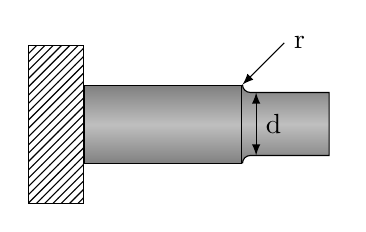
\begin{tikzpicture}[>=latex]
    \node [draw, top color=Grey, bottom color=Grey, middle color=Grey!50!White, rectangle, minimum height=1cm, minimum width=2cm](left){};
    \node at (left.west) [anchor=east, draw, pattern=north east lines, minimum height=2cm, minimum width=0.7cm](wall){};
    \draw [top color=Grey, bottom color=Grey, middle color=Grey!50!White,] (left.north east) arc (-180:-90:0.1) --++ (0:1) node(middle){} --++ (-90:0.8) --++ (180:1) arc (90:180:0.1);
    \draw [<-] (left.north east) --++ (45:0.75) node[right]{r};
    \draw [<->] (left.north east) ++ (-30:0.2) --++ (-90:0.8) node[midway, right]{d};
  \end{tikzpicture}
  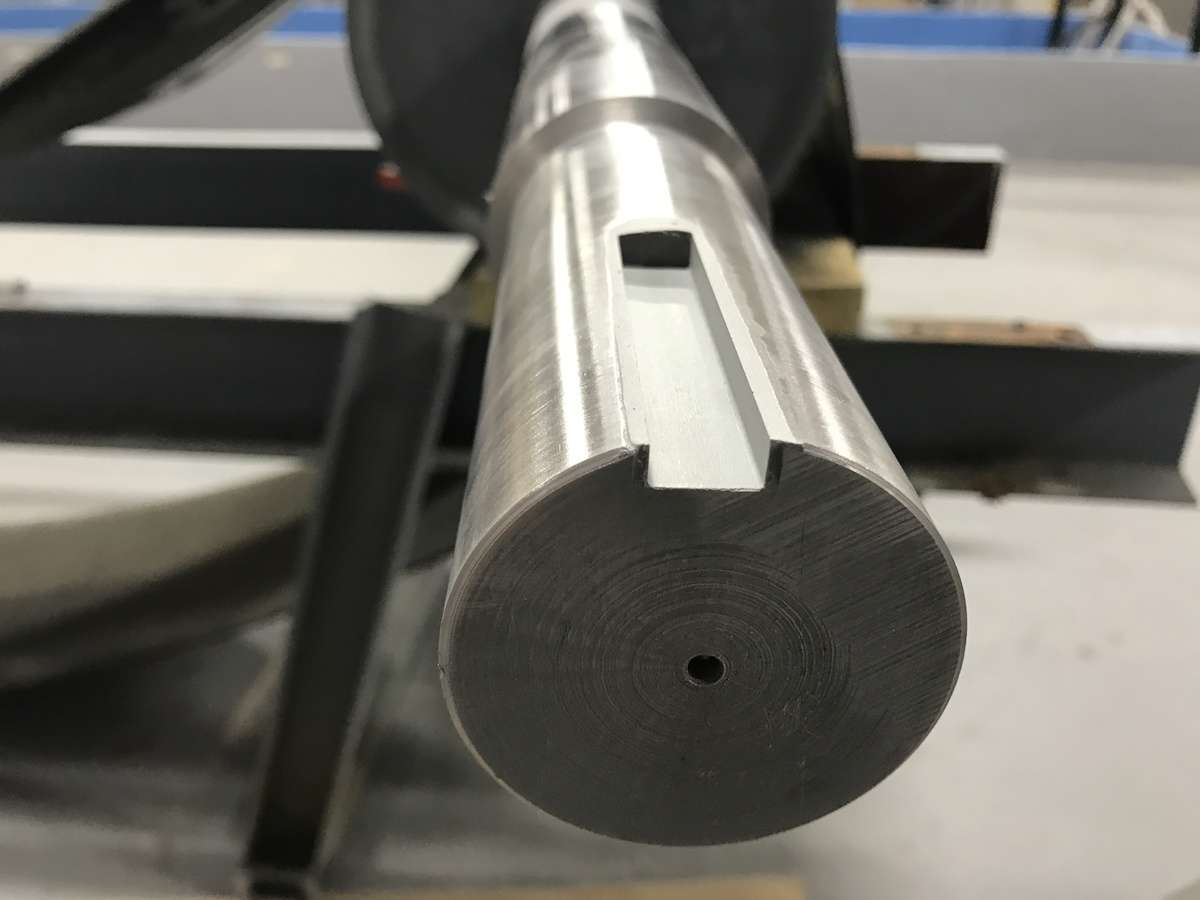
\includegraphics[height=0.25\textheight]{Pictures/keyseat}
  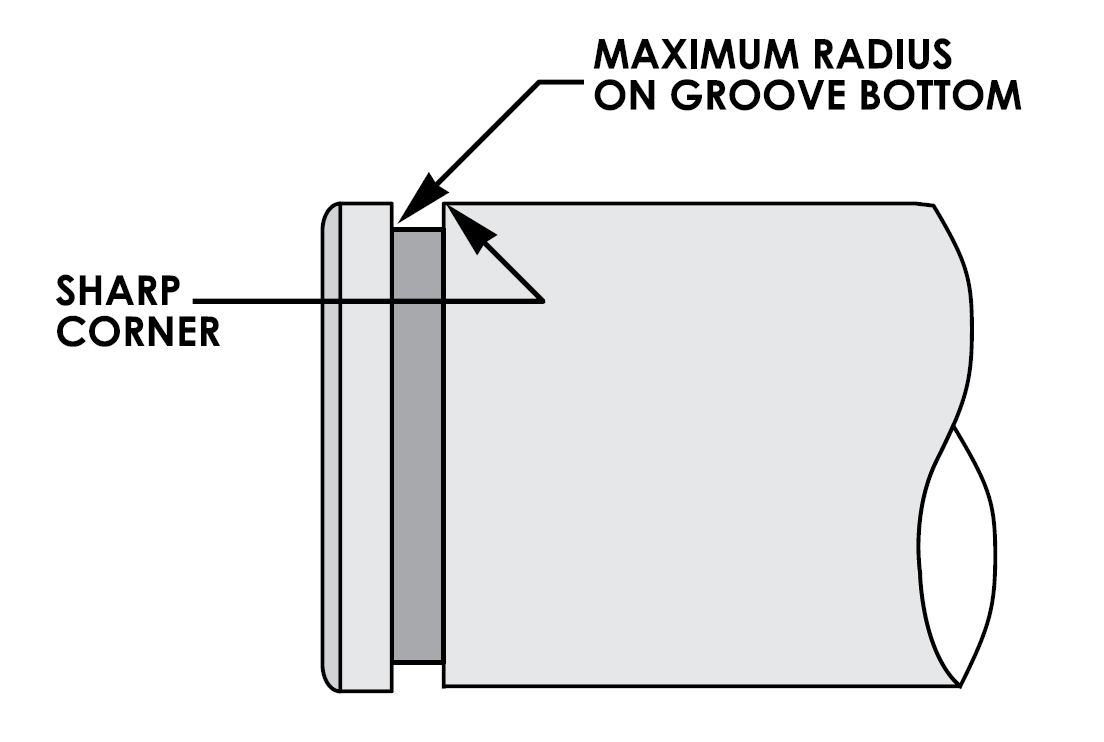
\includegraphics[height=0.25\textheight]{Pictures/retaining-ring-groove}
\end{figure}
\begin{table}[h]
  \centering
  \begin{tabular}{lccc}
    \toprule
     & Bending & Torsion & Axial \\
    \midrule
    Shoulder fillet---sharp ($r/d$ = 0.02) & 2.7 & 2.2 & 3.0 \\
    Shoulder fillet---well rounded ($r/d$ = 0.1) & 1.7 & 1.5 & 1.9 \\
    End-mill keyseat ($r/d$ = 0.02) & 2.14 & 3.0 & --- \\
    Sled runner keyseat  & 1.7 & --- & --- \\
    Retaining ring groove & 5.0 & 3.0 & 5.0 \\
    \bottomrule
  \end{tabular}
\end{table}
\end{frame}

\begin{frame}[label={sec:org99c9eba}]{Shaft Stresses}
\begin{itemize}
\item Torsion + Bending
\item Axial load usually small and negligible

\begin{align*}
  \sigma_{a} &= K_{f} \frac{ M_{a} c }{I} \hspace{1cm} \sigma_{m} = K_{f} \frac{M_{m} c}{I} \\
  \tau_{a} &= K_{fs} \frac{ T_{a} c }{J} \hspace{1cm} \tau_{m} = K_{fs} \frac{T_{m} c}{J}
\end{align*}
\end{itemize}
\end{frame}

\begin{frame}[label={sec:org6d82404}]{Solid round shafts}
\begin{align*}
  \sigma_{a} &= K_{f} \frac{ 32 M_{a}}{\pi d^{3}} \hspace{1cm} \sigma_{m} = K_{f} \frac{32M_{m}}{\pi d^{3}} \\[10pt]
  \tau_{a} &= K_{fs} \frac{ 16T_{a}}{\pi d^{3}} \hspace{1cm} \tau_{m} = K_{fs} \frac{16 T_{m}}{\pi d^{3}}
\end{align*}
\end{frame}

\begin{frame}[label={sec:org406d0fc}]{Combine Normal and Shear Stresses}
Use MDET
\begin{align*}
  \sigma_{e} &= \left( \sigma^{2} + 3 \tau^{2} \right)^{1/2} \\
  \sigma_{ae} &= \left( \sigma_{a}^{2} + 3 \tau_{a}^{2} \right)^{1/2} = \left[ \left( \frac{32 K_{f} M_{a}}{\pi d^{3}} \right)^{2} + 3 \left( \frac{16 K_{fs} T_{a}}{\pi d^{3}} \right)^{2} \right]^{1/2} \\
  \sigma_{me} &= \left( \sigma_{m}^{2} + 3 \tau_{m}^{2} \right)^{1/2} = \left[ \left( \frac{32 K_{f} M_{m}}{\pi d^{3}} \right)^{2} + 3 \left( \frac{16 K_{fs} T_{m}}{\pi d^{3}} \right)^{2} \right]^{1/2}
\end{align*}
\end{frame}

\begin{frame}[label={sec:orgec9221b}]{Apply Fatigue Limit}
\small
\begin{align*}
  \frac{1}{N_{s}} &= \frac{\sigma_{ae}}{S_{e}} + \frac{\sigma_{me}}{S_{y}} \\
  \frac{1}{N_{s}} &= \frac{16}{\pi d^{3}} \left\{ \frac{1}{S_{e}} \left[ 4 \left( K_{f} M_{a} \right)^{2} + 3 \left( K_{fs} T_{a} \right)^{2} \right]^{1/2} + \frac{1}{S_{y}} \left[ 4 \left( K_{f} M_{m} \right)^{2} + 3 \left( K_{fs} T_{m} \right)^{2} \right]^{1/2} \right\} \\[2em]
  d &= \left( \frac{16 N_{s}}{\pi} \left\{ \frac{1}{S_{e}} \left[ 4 \left( K_{f} M_{a} \right)^{2} + 3 \left( K_{fs} T_{a} \right)^{2} \right]^{1/2} + \frac{1}{S_{y}} \left[ 4 \left( K_{f} M_{m} \right)^{2} + 3 \left( K_{fs} T_{m} \right)^{2} \right]^{1/2} \right\} \right)^{1/3}
\end{align*}
\end{frame}

\begin{frame}[label={sec:org52a22db}]{Shaft Loading Conditions}
\begin{itemize}
\item Torque
\item Bending \(\implies\) radial load from torque transmission
\end{itemize}

\centering
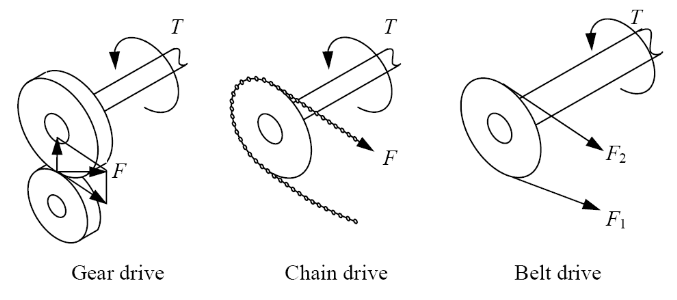
\includegraphics[width=0.8\textwidth]{Pictures/torque-transmission}
$$ F = \dfrac{T}{r \cos \theta} \hspace{1cm} F = \dfrac{T}{r} \hspace{1cm} F_2 - F_1 = \dfrac{T}{r} $$
\end{frame}

\begin{frame}[label={sec:org0fe2dbf}]{Example: Timing Belt Shaft}
Size the shaft (AISI 1040, \(S_y\) = 400 MPa, \(S_{ut}\) = 600 MPa) using

\begin{enumerate}
\item MDET (Static Loading)
\item Soderberg theory (Dynamic Loading)

Take \(r_{\text{pulley}}\) = 10 cm and \(N_{s}\) = 3

\begin{center}
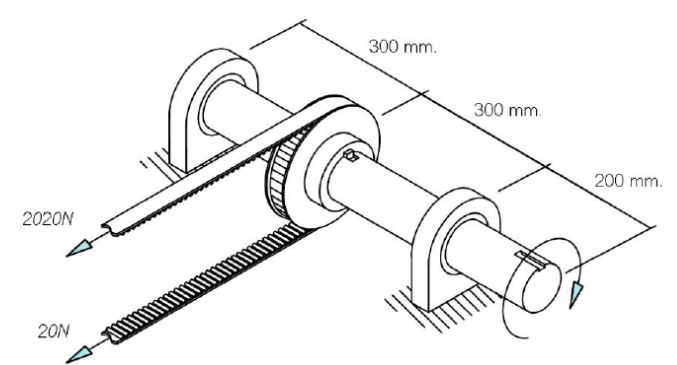
\includegraphics[width=.9\linewidth]{./Pictures/shaft-sizing.png}
\end{center}
\end{enumerate}
\end{frame}

\begin{frame}[label={sec:orga3b396e}]{}
\begin{itemize}
\item The applied torque \(T\) is \((2020 - 20)(0.1) = 200\) N-m.
\item Midpoint load of 2020 + 20 = 2040 N
\item Assuming end-mill keyseat at the sheave: \(K_{f}\) = 2.14, \(K_{fs}\) = 3
\end{itemize}
\end{frame}

\begin{frame}[label={sec:orgf2a7c2e}]{Calculating Stresses}
\begin{align*}
  M &= \frac{FL}{4} = \frac{2040(0.6)}{4} = 306 \\
  \sigma_{bending} &= K_{f}\frac{My}{I} = 2.14 \frac{306(d/2)}{(\pi/4) (d/2)^{4}} = \frac{6670}{d^{3}} \\
  \tau_{T} &= K_{fs}\frac{Tr}{J} = 3 \frac{200(d/2)}{(\pi/2)(d/2)^{4}} = \frac{3056}{d^{3}}
\end{align*}
\end{frame}

\begin{frame}[label={sec:orga3c7bfd}]{Applying MDET}
Using MDET, we have that
\begin{align*}
  \sigma_{e} &= \sqrt{\left(\frac{6670}{d^{3}}\right)^{2} + 3\left(\frac{3056}{d^{3}}\right)^{2}} = \frac{8514}{d^{3}}\\
  N_{s} &= 3 = \frac{S_{y}}{\sigma_{e}} = \frac{400 \times 10^{6}}{\sigma_{e}} \\
  d^{3} &= \frac{8514}{400 \times 10^{6}} = 2.13 \times 10^{-5} \\
  d &= 0.0277
\end{align*}
\end{frame}

\begin{frame}[label={sec:orgc817622}]{Applying Soderberg}
\begin{itemize}
\item Bending \(\rightarrow\) repeated stress (tensile and compressive)
\item \(\sigma_{a} = \sigma_{bending}\), \(\sigma_{m} = 0\)
\item Torsion \(\rightarrow\) constant stress
\item \(\tau_{a} = 0, \tau_{m} = \tau_{T}\)
\end{itemize}


\begin{align*}
  \sigma_{ae} &= \sqrt{\sigma_{a}^{2} + 3\tau_{a}^{2}} = \sigma_{bending} \\
  \sigma_{me} &= \sqrt{\sigma_{m}^{2} + 3\tau_{m}^{2}} = \sqrt{3}\tau_{T}
\end{align*}
\end{frame}

\begin{frame}[label={sec:orgf5b986a}]{Applying Soderberg II}
\begin{align*}
  \frac{1}{N_{s}} &= \frac{1}{3} = \frac{\sigma_{ae}}{S_{e}} + \frac{\sigma_{me}}{S_{y}} = \frac{6670}{d^{3}(0.5)(600 \times 10^{6})} + \frac{\sqrt{3}(3056)}{d^{3}(400 \times 10^{6})}\\
  d^{3} &= 1.06 \times 10^{-4} \\
  d &= 0.0474
\end{align*}
\end{frame}

\begin{frame}[label={sec:org0d4228d}]{General Guidelines}
\begin{enumerate}
\item shaft should be as short as possible
\item avoid sharp step
\item round shaft if possible
\item to save weight \(\rightarrow\) hollow shaft
\end{enumerate}
\end{frame}

\section{Deflection Analysis}
\label{sec:org08cc75c}

\begin{frame}[label={sec:org4284ec7}]{Deflection Considerations}
\begin{itemize}
\item Need geometry for entire shaft
\item Should evaluate at gears and bearings -- why?
\item Maximum deflection < gear teeth size
\item In most case, software is needed
\end{itemize}
\end{frame}

\section{Critical Speeds for Shafts}
\label{sec:org0300b55}

\begin{frame}[label={sec:orge4ac8aa}]{Shaft Whirling or Shaft Whip}
\begin{itemize}
\item At high speed, the centrifugal force can cause shaft deflection \(\sim\) buckling
\item For simple shafts:
\begin{align*}
  \omega_{1} = \left( \frac{\pi}{l} \right)^{2} \sqrt{ \frac{EI}{m} } = \left( \frac{\pi}{l} \right)^{2} \sqrt{ \frac{EI}{A \rho} }
\end{align*}

\begin{description}
\item[{\(m\)}] mass per unit length
\item[{\(\rho\)}] density
\item[{\(E\)}] Young's modulus
\item[{\(A\)}] cross-sectional area
\end{description}
\end{itemize}
\end{frame}

\begin{frame}[label={sec:org0782419}]{Example: Resize the Shaft}
From previous example, use \(E\) = 210 GPa and reconsider the proper shaft size if \(\omega_{\max}\) = 10000 rpm

\vfill
\end{frame}

\section{Torque Transmission Components}
\label{sec:org974b792}

\begin{frame}[label={sec:org398dfea}]{Torque Transmission}
\begin{figure}[htbp]
  \centering
  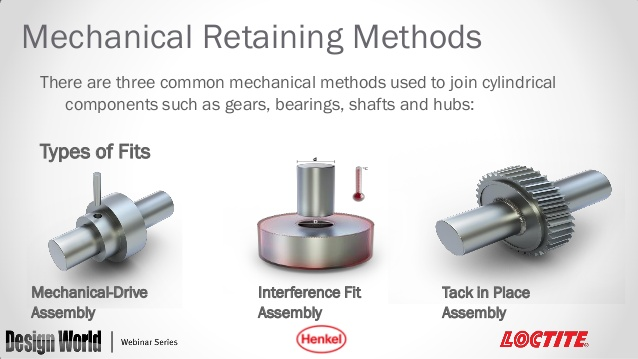
\includegraphics[width=0.8\textwidth]{Pictures/types-of-fits}
\end{figure}

\begin{itemize}
\item Mechanical drive assembly
\item Interference fit assembly
\item Welded assembly
\end{itemize}
\end{frame}

\begin{frame}[label={sec:org4427caa}]{Mechanical Drive Assembly}
\begin{figure}[htbp]
  \centering
  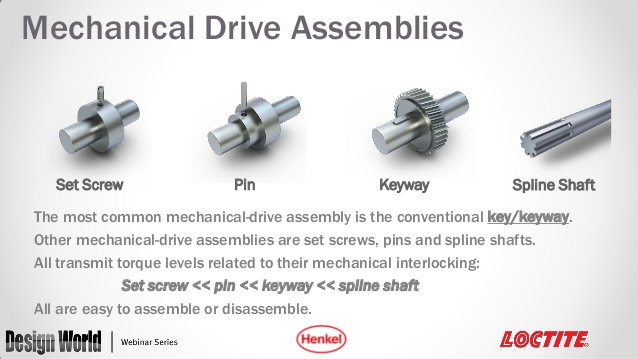
\includegraphics[width=\textwidth]{Pictures/mech-drive}
\end{figure}
\%
\%       - Set screw
\%       - Pin
\%       - Key
\%       - Spline shaft
\%


** Setscrews\}

\begin{itemize}
\item Use friction to hold a component on the shaft \(\rightarrow\) \emph{holding power} (\(H\))
\item Torque capacity can be calculated by
\begin{align*}
  T_{\max} = Hr_{\text{shaft}}
\end{align*}
\end{itemize}

\begin{figure}[htbp]
  \centering
  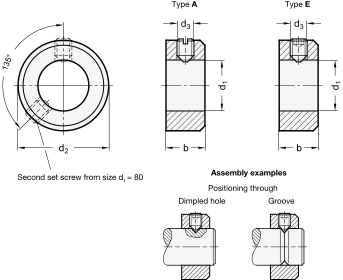
\includegraphics[width=0.6\textwidth]{Pictures/set-screws}
\end{figure}


** Setscrew Sizes\}
\begin{table}[htbp]
  \centering
  \begin{tabular}{lll}
    \toprule
    Thread size & Tightening Torque (N) & Holding Power (N) \\
    \midrule
    M3 & 0.87 & 710 \\
    M4 & 2.20 & 1700 \\
    M5 & 4.60 & 2500 \\
    M6 & 7.80 & 4200 \\
    M8 & 18.00 & 6700 \\
    M10 & 36.00 & 9300 \\
    M12 & 62.00 & 12000 \\
    M16 & 150.00 & 18000 \\
    M20 & 290.00 & 23000 \\
    \bottomrule
  \end{tabular}
\end{table}


** Keys and pins\}

\begin{itemize}
\item Keys allow torque transmission
\item Pins allow axial positioning, torque and thrust transfer
\end{itemize}

\begin{figure}[htbp]
  \centering
  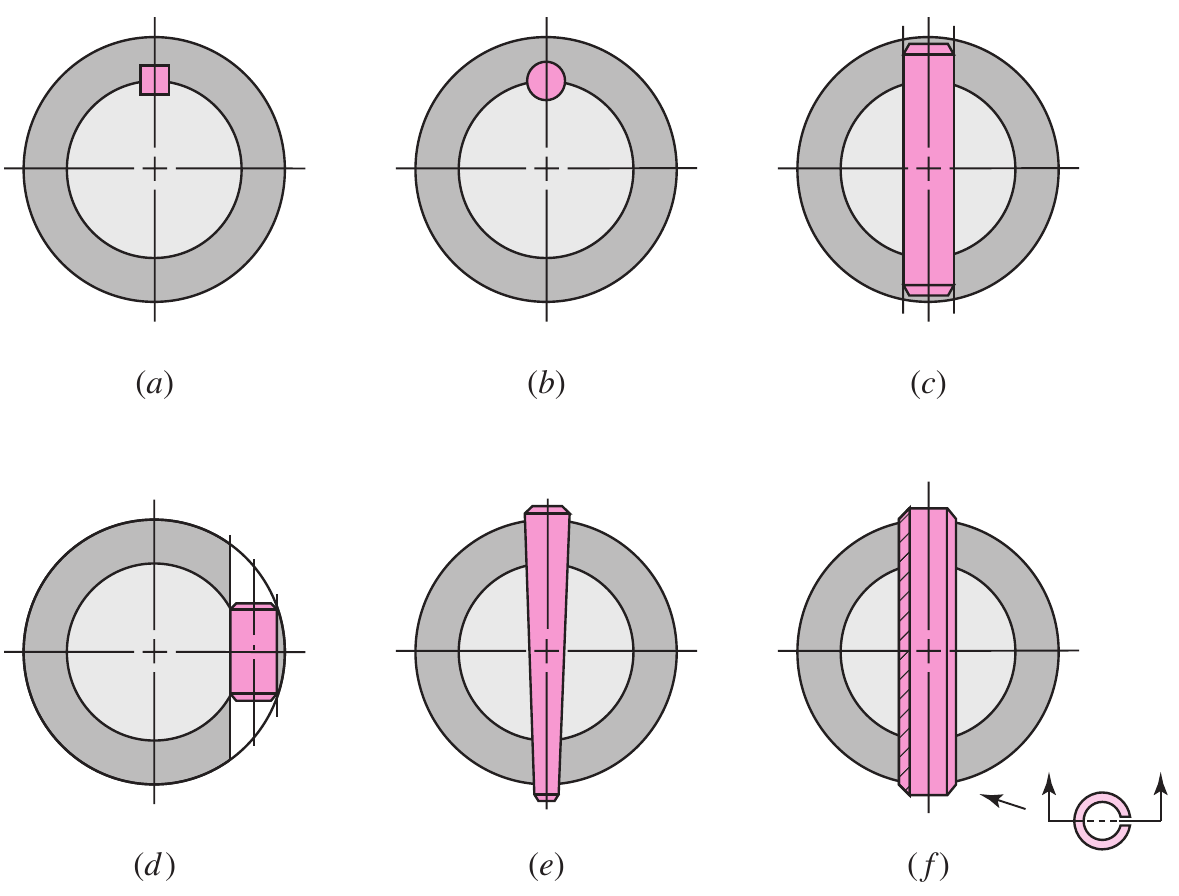
\includegraphics[width=0.8\textwidth]{Pictures/keys-pins}
\end{figure}


** Key and Pin Capacity\}

\begin{itemize}
\item Axial load and torque capacity depends on key/pin strength and its cross section.
\begin{align*}
  P_{\max} &= \frac{S_{y}}{\sqrt{3}}A = 0.577S_{y}A \\
  T_{\max} &= P_{\max}r_{\text{shaft}}
\end{align*}

\item Key length \(\leqslant 3r_{\text{shaft}}\) to ensure even load distribution during torsion
\end{itemize}
\end{frame}

\begin{frame}[label={sec:org6a3b8ec}]{Example: Key sizing}
A steel shaft whose \(S_{y}\) = 450 MPa has a radius of 5 cm. The shaft rotates at 600 rpm and transmits 40 hp through a gear. Select and appropriate key for the gear. Use safety factor = 3.

\begin{figure}[htbp]
  \centering
  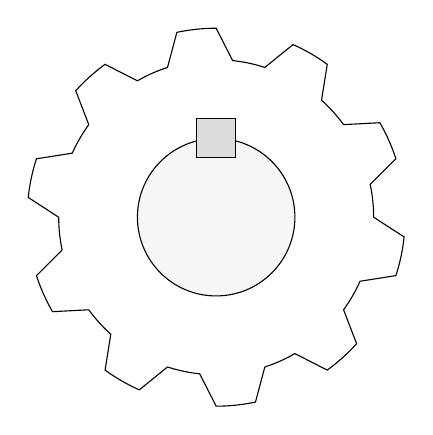
\begin{tikzpicture}
    \node[circle, draw, fill=LightGrey!20, minimum height=2cm](shaft){};
    \draw
    \foreach \i in {1,2,...,10} {%
      [rotate=(\i-1)*36]  (0:2)  arc (0:12:2) -- (18:2.4)  arc (18:30:2.4) --  (36:2)
    };
    \node at (shaft.north) [draw, fill=LightGrey!80, minimum height=5mm, minimum width=5mm](key){};
  \end{tikzpicture}
\end{figure}
\end{frame}

\begin{frame}[label={sec:orga639a17}]{Solution: Key sizing}
To keep things simple, pick a square key and pick key length = 2 cm.

\begin{align*}
  T &= \frac{\text{Power}}{\omega} = \frac{40(746)}{600(2\pi/60)} \\
    &= 475 \text{ N-m}
\end{align*}

For the width (and height) of the key section,

\begin{align*}
  N_{s} T_{\max} &= 0.577S_{y}blr_{\text{shaft}} \\
  b &= \frac{3(475)}{0.577(450 \times 10^{6})(0.02)(0.05)} \\
  b &= 0.00549 \text{ m}
\end{align*}


** Retaining Rings\}

\begin{itemize}
\item Used to axially locate a component on a shaft or a hub.
\item Need  to cut grooves in shaft to fit \(\rightarrow\) stress concentration
\end{itemize}

\begin{figure}[htbp]
  \centering
  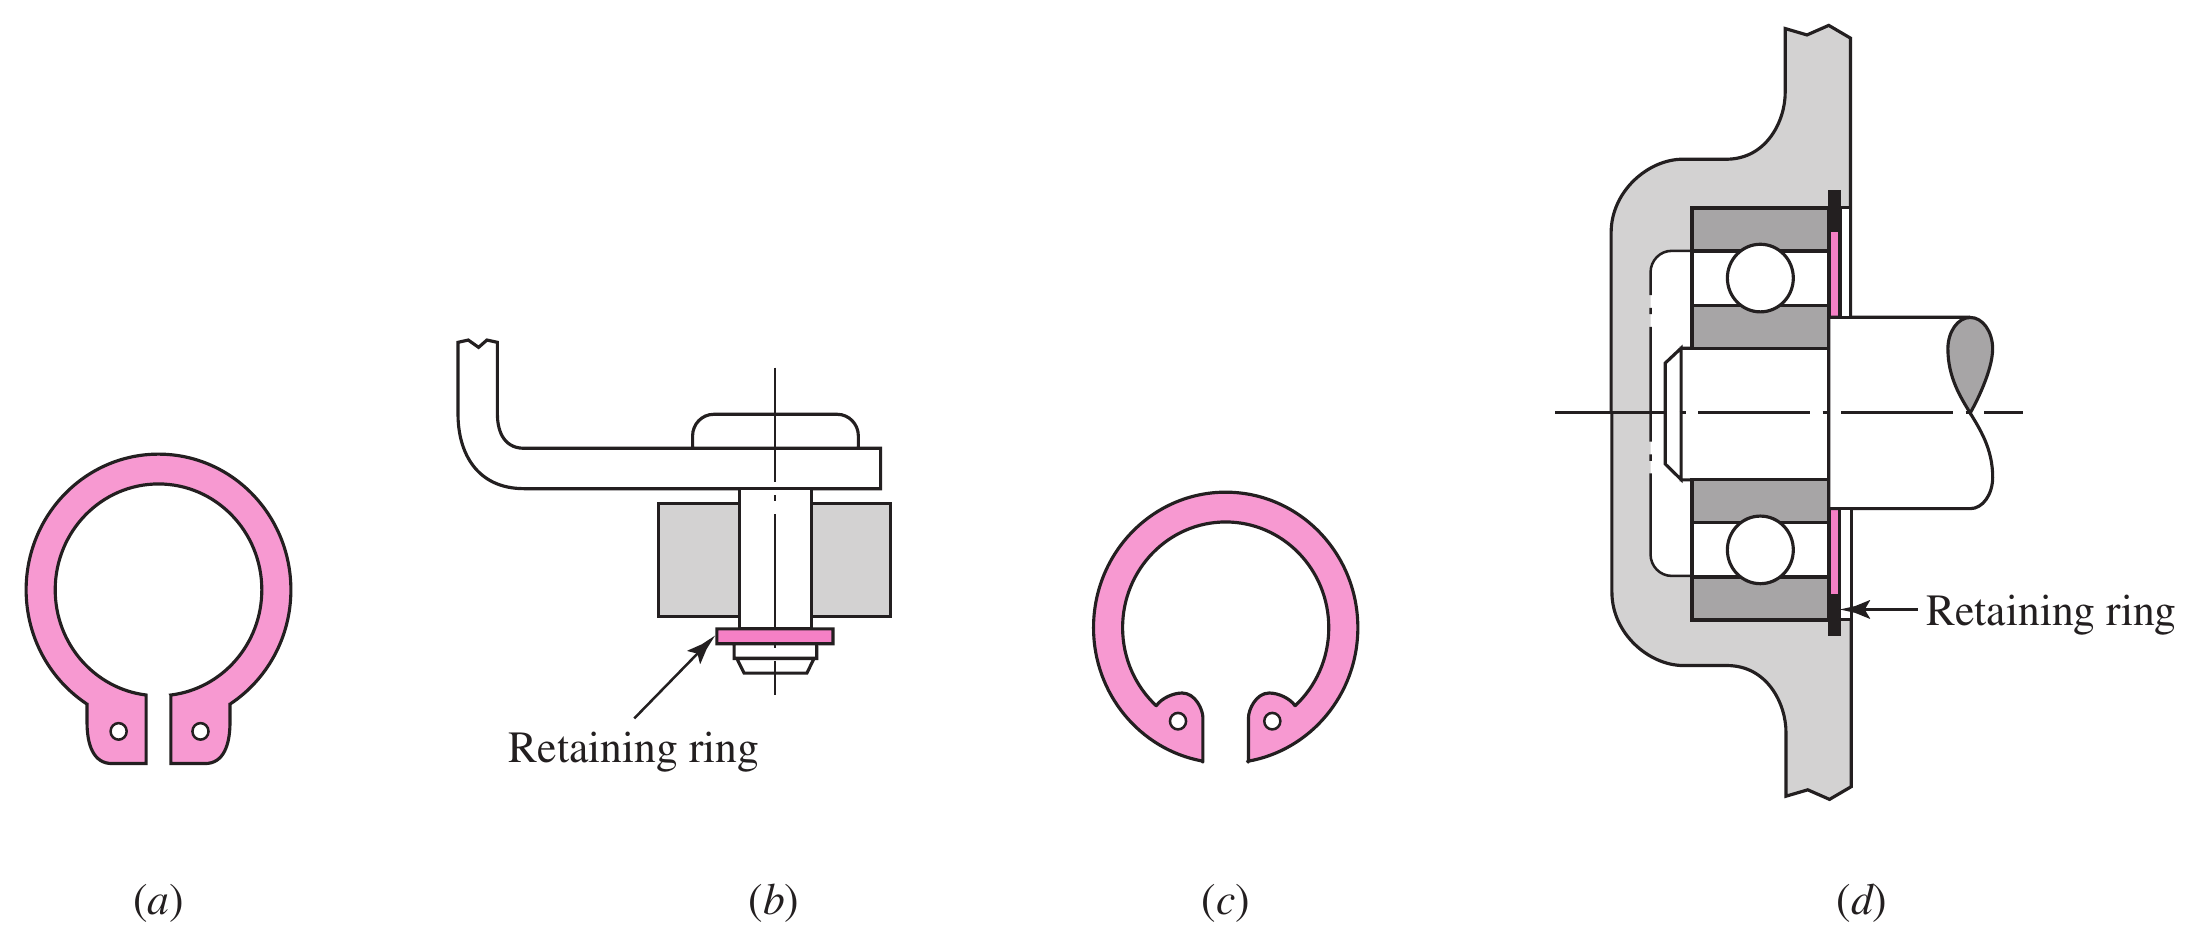
\includegraphics[width=\textwidth]{Pictures/retaining-rings}
\end{figure}
\end{frame}

\begin{frame}[label={sec:org053e2dc}]{Limitation of Mechanical Drive}
\begin{itemize}
\item Stress concentration
\item Backlash
\item Machining costs
\item Uneven distribution of mass
\end{itemize}
\end{frame}

\begin{frame}[label={sec:org4aa2a2b}]{Interference Fit Assemblies}
\begin{itemize}
\item Press fit: \(d_{\text{shaft}} > d_{\text{hub}}\)
\item Tapered fit: Taper + Fastener = Fit
\item Shrink fit: Hole is heated or shaft is cooled before assembly
\item Used to minimize need for shoulders and keyways
\end{itemize}
\end{frame}

\begin{frame}[label={sec:org0958ef7}]{Limitations of Interference Fits}
\begin{itemize}
\item Material, surface, and design restrictions -- need sufficient friction
\item Close tolerance \(\rightarrow\) high machining costs
\item Micro-movement causes fretting corrosion
\item Surface galling \(\rightarrow\) difficult disassembly
\item High stress in components
\end{itemize}
\end{frame}

\begin{frame}[label={sec:orga5c62f3}]{Stress in Interference Fits}
\begin{itemize}
\item Assumed uniform pressure on shaft and hub
\end{itemize}


\begin{align*}
  p &= \frac{d_{\text{shaft}} - d_{\text{hub}}}{\dfrac{d}{E_{o}} \left( \dfrac{d_{o}^{2} + d^{2}}{d_{o}^{2} - d^{2}} + \nu_{o} \right) + \dfrac{d}{E_{i}}\left( \dfrac{d^{2} + d_{i}^{2}}{d^{2} - d_{i}^{2}} - \nu_{i} \right)}
\end{align*}


\begin{itemize}
\item When both are of the same material
\end{itemize}


\begin{align*}
  p &= \frac{E(d_{\text{shaft}} - d_{\text{hub}})}{2d^{3}} \left[ \frac{(d_{o}^{2} - d^{2})(d^{2} - d_{i}^{2})}{d_{o}^{2} - d_{i}^{2}} \right]
\end{align*}

\begin{description}
\item[{\(d\)}] nominal shaft diameter
\item[{\(d_{i}\)}] inside diameter of shaft
\item[{\(d_{o}\)}] outside diameter of hub
\end{description}
\end{frame}

\begin{frame}[label={sec:orga42486d}]{Stress in Interference Fits}
\begin{itemize}
\item Tangential and radial stresses in shaft and hub are

\begin{align*}
  \sigma_{t,\text{shaft}} &= -p \frac{d^{2} + d_{i}^{2}}{d^{2} - d_{i}^{2}} \\
  \sigma_{t,\text{hub}} &= p \frac{d_{o}^{2} + d^{2}}{d_{o}^{2} - d^{2}} \\
  \sigma_{r,\text{shaft}} &= -p \\
  \sigma_{r,\text{hub}} &= -p
\end{align*}

\item Combine \(\sigma_{t}\) and \(\sigma_{r}\) using MDET to determine failure
\end{itemize}
\end{frame}

\begin{frame}[label={sec:org0038139}]{Torque Capacity in Interference Fits}
\begin{itemize}
\item Depends on friction generated between shaft and hub \(\rightarrow\) pressure from interference fits
\end{itemize}


\begin{align*}
  f &= \mu N = \mu (pA) \\
    &= \pi \mu pld \\
  T &= fd/2 = \pi \mu pld(d/2) \\
    &= \frac{\pi}{2}\mu pld^{2}
\end{align*}
\end{frame}

\begin{frame}[label={sec:org0676c93}]{Example: Torque Capacity of a Gear on a Shaft}
A solid shaft whose diameter is 5 cm is pressed onto a gear whose hub inner diameter is 4.99 cm and outer diameter is 6 cm. If both are made of the same steel whose \(E\) = 210 GPa and \(\nu\) = 0.3, determine the radial and tangential stresses, along with the torque capacity of the fit. Assume steel-on-steel \(\mu\) = 0.3, and the hub is 7 cm long.
\end{frame}

\begin{frame}[label={sec:org9b96f64}]{Solution: Torque Capacity of a Gear on a Shaft}
\begin{align*}
  p &= \frac{E(d_{\text{shaft}} - d_{\text{hub}})}{2d^{3}} \left[ \frac{(d_{o}^{2} - d^{2})(d^{2} - d_{i}^{2})}{d_{o}^{2} - d_{i}^{2}} \right] \\
    &= \frac{210 \times 10^{9} (0.05 - 0.0499)}{2(0.05)^{3}} \left[ \frac{(0.06^{2} - 0.05^{2})(0.05^{2} - 0)}{0.06^{2} - 0} \right] \\
    &= 64.2 \text{ MPa} \\
  \sigma_{r,\text{shaft}} &= \sigma_{r,\text{hub}} = -64.2 \text{ MPa} \\
  \sigma_{t,\text{shaft}} &= -64.2 \frac{0.05^{2}}{0.05^{2}} = -64.2 \text{ MPa} \\
  \sigma_{t,\text{hub}} &= 64.2 \frac{0.06^{2} + 0.05^{2}}{0.06^{2} - 0.05^{2}} = 356 \text{ MPa} \\
  T &= \frac{\pi}{2}\mu pld^{2} = \frac{\pi}{2}(0.3) 64.2 \times 10^{6} (0.07)(0.05^{2}) = 5294 \text{ N-m}
\end{align*}
\end{frame}

\begin{frame}[label={sec:org83fee6e}]{Welded Assembly}
\begin{figure}[htbp]
  \centering
  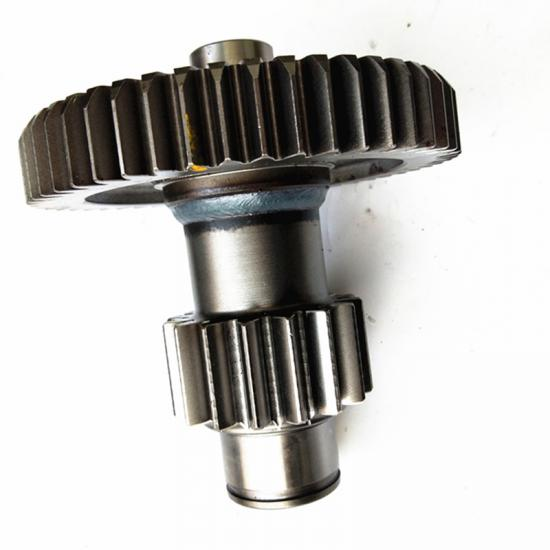
\includegraphics[width=0.5\textwidth]{Pictures/welded-shaft}
\end{figure}

\begin{itemize}
\item Connections by welding the part
\item Load carried by small welded area
\end{itemize}
\end{frame}

\begin{frame}[label={sec:orge573f5c}]{Limitations of welded assembly}
\begin{itemize}
\item Only compatible materials
\item Heating can cause warpage
\item Difficult disassembly
\item Additional costs
\item Need skilled personnel
\item Addtional cleaning and grinding afterwards
\end{itemize}
\end{frame}
\end{document}